\Author{\daAuthorOne}

\todo{Bilder bearbeiten, weil gerade keine Daten angezeigt werden beim deployten Admin-Panel}

The Admin Panel is a Flutter-based administrative dashboard that allows the administrator to efficiently manage all addresses in the application, to plan  future "Sternsinger" events and assign designated zones to groups. This zoning ensures organized distribution of participants. It enables CRUD (Create, Read, Update, Delete) operations on addresses, streets and zones. These features make it easy for the administrator to quickly address issues and make changes to areas that participants need to visit.

\subsection{Navigation}

\noindent

\begin{figure}[H]

\begin{minipage}{0.58\textwidth}
    \setstretch{1.5} % Erhöht den Zeilenabstand
    The file \texttt{AdminNavigation} is used to navigate between the different pages of the Admin Panel. The navigation can be done via a sidebar on the left which can be set visible via a button on the top left of the screen. The widget contains a list of pages and maintains an internal state (\texttt{indexState}) to keep track of the currently selected page. Whenever a page is selected in the sidebar, the \texttt{indexState} is updated and the corresponding page is displayed.
    \end{minipage}
    \hfill
    \begin{minipage}{0.38\textwidth}
    \centering
    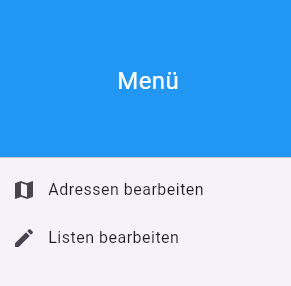
\includegraphics[width=0.7\linewidth]{images/AdminPanel/Menu.png}
    \caption{Navigation in Admin-Panel}
    \label{fig:adminpanel_navigation}
\end{minipage}

\end{figure}




\begin{subsection}{AddressPage}

The \texttt{AddressPage} displays all addresses in the database. With it, the administrator can add, edit and delete addresses into the database. All addresses are shown either in the \texttt{MapComponent} or the \texttt{DatabaseViewComponent} on the right. On the left of the page are \texttt{InputFields} (\ref{fig:InputField}), which are used to enter new information about a new address, or edit an existing one. Overlapping the \texttt{MapComponent} there are:
\begin{itemize}
  \item a field to filter the addresses displayed
  \item a button with a dropdown menu to select an edit a street
  \item a switch to toggle between the \texttt{MapComponent} and the \texttt{DatabaseViewComponent}
  \item a information box on the bottom left corner to display the selected coordinates, which is only visible when the admin presses the map
\end{itemize}

\begin{figure}[H]
    \centering
    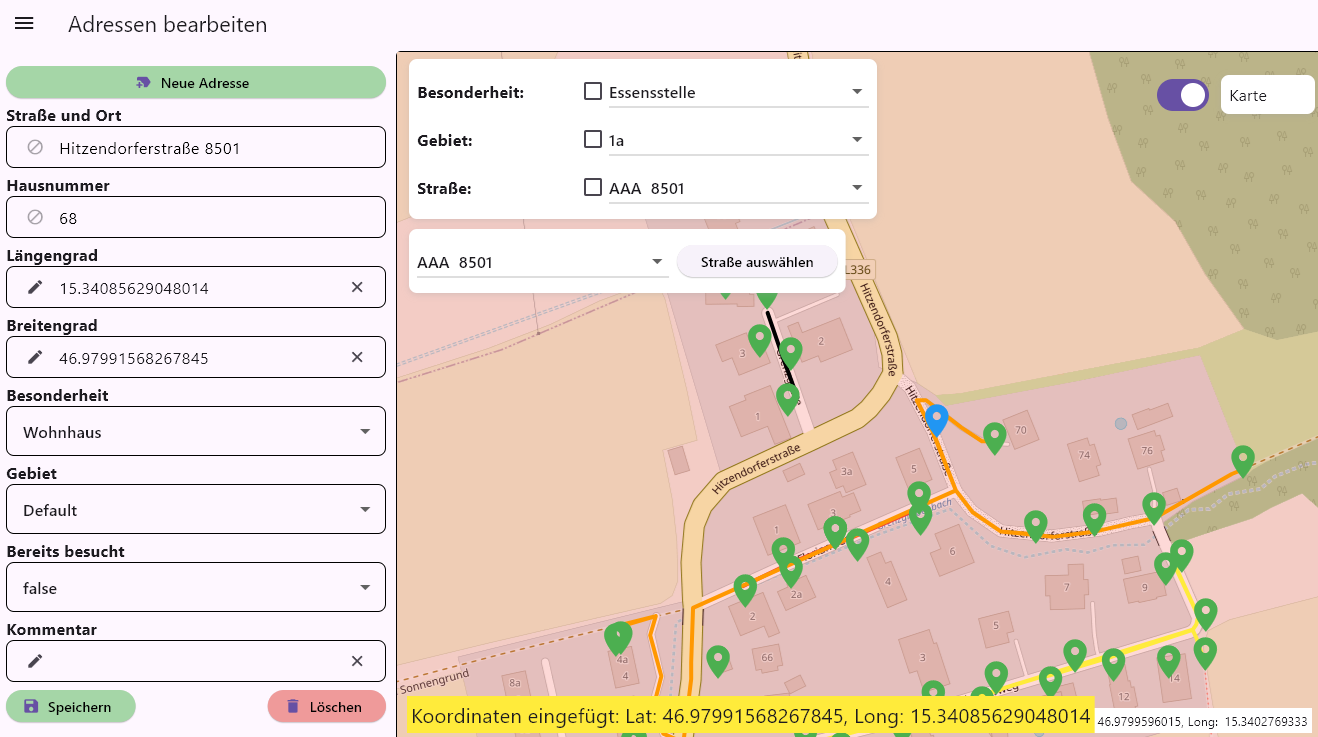
\includegraphics[width=0.9\linewidth]{images/AdminPanel/AddressPage.png}
    \caption{AddressPage}
\end{figure}
\end{subsection}

\label{fig:Add Address}
\subsubsection{Add Address}
To add a new address, the button "Neue Adresse" is pressed. This triggers the \texttt{onClickNewAddress} method, which clears all \texttt{InputFields} and sets the boolean variable \texttt{isNewAddress} to \texttt{true}. This variable indicates that a new address is being saved. The cleared fields can then be filled with the new address information.\\When the "Speichern" button is pressed, the \texttt{saveAddress} method is called. This method performs validation checks and verifies whether the address already exists in the database. If the address is valid and not a duplicate, the \texttt{AdminAddressProvider} is called to add the new address to the database.

% \lstset{style=mycsharp, caption=saveAddress method}
% \begin{lstlisting}
%     void saveAddress(AdminAddressProvider provider) async {
%     if (selectedAddresses.isEmpty) return;
%     if (isNewAddress) {
%       Address newAddress = createAddressFromInput();
%       if (!validateAddressFields(newAddress)) return;
%       newAddress.area = provider.areas.firstWhere((a) => a.desc == newAddress.area.desc);
%       newAddress.specialFeature = provider.specialFeatures.firstWhere((s) => s.text == newAddress.specialFeature.text);
%       if (selectedAddresses.length == 1) {
%         newAddress.street = provider.streets.firstWhere(
%           (s) => s.name == newAddress.street.name && s.postalCode == newAddress.street.postalCode,
%         );
%       }
%       if (isDuplicateAddress(provider.addresses, newAddress)) {
%         showNotification("Adresse existiert bereits", () => showAddAddressNotification = true);
%         return;
%       }
%       if (await provider.addAddress(newAddress) == 200) {
%         showNotification("Adresse hinzugefuegt", () => showAddAddressNotification = true);
%       }
%     } else {
%       selectedAddresses.length > 1 ? updateMultipleAddresses(provider) : updateSingleAddress(provider);
%     }
%   }
% \end{lstlisting}

\subsubsection{Edit Address}
\sloppy % Damit der Text (\texttt{DatabaseViewComponent}) nicht über den Rand hinausragt
Existing addresses can be edited, by selecting an address in the \texttt{MapComponent} or the \texttt{DatabaseViewComponent}. The \texttt{InputFields} are then filled with the information of the selected address and however, in this case, the boolean variable \texttt{isNewAddress} is set to \texttt{false}, to indicate that an existing address or addresses are being updated. The admin can then edit the information and press the "Speichern" button. This triggers the \texttt{saveAddress} method, which performs the same validation checks as when adding a new address. The \texttt{AdminAddressProvider} updates the selected addresses in the database.

\subsubsection{Delete Address}
After selecting addresses in the \texttt{MapComponent} or the \texttt{DatabaseViewComponent}, the admin can press the "Löschen" button to delete them. This triggers the \texttt{deleteAddress} method, which calls the \texttt{AdminAddressProvider} to delete the selected addresses.\\The method also triggers the \texttt{showDeleteDialog} method, which displays a \texttt{AlertDialog} to confirm the action to prevent accidental deletions.

\begin{figure}[H]
    \centering
    
\includegraphics[width=0.6\linewidth]{images/AdminPanel/DeleteDialog.png}
    \caption{Dialog to confirm deletion}
\end{figure}

\subsubsection{Validation}
Validation is the process of checking that data meets specific criteria before it is accepted and added. It is crucial to ensure that the data entered is correct.
\paragraph{isDuplicateAddress}
To determine whether an edited or newly added address already exists, All addresses are compared with the new address. It is called in the \texttt{saveAddress} method.  If it already exists, the method returns \texttt{true}, otherwise \texttt{false}. A duplicate address is identified by the following criteria:
\begin{itemize}
    \item street name
    \item postal code
    \item house number
\end{itemize}

\lstset{style=mycsharp, caption=isDuplicateAddress method}
\begin{lstlisting}
    bool isDuplicateAddress(List<Address> existingAddresses, Address newAddress) {
        return existingAddresses.any((existing) =>
            existing.street.name == newAddress.street.name &&
            existing.street.postalCode == newAddress.street.postalCode &&
            existing.houseNumber == newAddress.houseNumber
        );
    }
\end{lstlisting}

\paragraph{validateAddressFields}
To make sure that all \texttt{InputFields} are filled, the \texttt{validateAddressFields} is called in the \texttt{saveAddress}(\ref{fig:Add Address}) method. This method needs an \texttt{Address}. So first an new \texttt{Address} is made and passed to \texttt{validateAddressFields}. It checks if all fields are filled and returns \texttt{true} if they are, otherwise \texttt{false}.

\lstset{style=mycsharp, caption=InputFormatter in Inputfield}
\begin{lstlisting}
    bool validateAddressFields(Address address) {
        if (address.street.name.isEmpty) {
            showNotification("Strasse fehlt", () => showAddAddressNotification = true);
        } else if (address.houseNumber.isEmpty) {
            showNotification("Hausnummer fehlt", () => showAddAddressNotification = true);
        } else if (address.specialFeature.text.isEmpty) {
            showNotification("Besonderheit fehlt", () => showAddAddressNotification = true);
        } else if (address.area.desc.isEmpty) {
            showNotification("Gebiet fehlt", () => showAddAddressNotification = true);
        } else if (address.latitude == 0.0 || address.longitude == 0.0) {
            showNotification("Koordinaten fehlen", () => showAddAddressNotification = true);
        } else {
            return true;
        }
        return false;
    }
\end{lstlisting}


\paragraph{InputField Validation}
The \texttt{InputField} validates \textbf{latitude} and \textbf{longitude} inputs to ensure their correctness. Validation is applied only when the \texttt{isNumberInput} parameter is set to true. If that is the case, then the \texttt{inputFormatter} is passed to the \texttt{textfield} to validate the input. This \texttt{inputFormatter} guarantees that only valid inputs are accepted, preventing incorrect entries. These are the three validators used in the \texttt{InputField}:

\begin{itemize}
    \item The first \texttt{FilteringTextInputFormatter} allows only numbers and dots.
    \item The first \texttt{TextInputFormatter} checks if the input contains more than one dot.
    \item The second \texttt{TextInputFormatter} guarantees that there are no more than three digits before the decimal point.
\end{itemize}

\lstset{style=mycsharp, caption=InputFormatter in Inputfield}
\begin{lstlisting}
    inputFormatters: widget.isNumberInput == true
        ? <TextInputFormatter>[
            FilteringTextInputFormatter.allow(RegExp('[0-9.]')),
            TextInputFormatter.withFunction(
                (oldValue, newValue) {
                if (newValue.text.split('.').length - 1 > 1) {
                    return oldValue;
                }
                return newValue;
            }),
            TextInputFormatter.withFunction(
                (oldValue, newValue) {
                String text = newValue.text;
                if (text.isNotEmpty) {
                    final parts = text.split('.');
                    if (parts[0].length > 3) {
                    return oldValue;
                }
            }
            return newValue;
            }),
          ]
        : null,
\end{lstlisting}



\subsubsection{Additional Functionalities}


\label{fig:Notification}
\paragraph{Notification}
To inform the administrator about the success or failure of an operation, a \texttt{Notification} is displayed on the bottom left over the \texttt{MapComponent}. This notification appears when an address is added, edited, deleted, or when validation fails.


\begin{figure}[H]
    \centering
    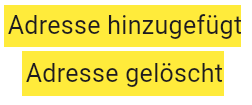
\includegraphics[width=0.4\linewidth]{images/AdminPanel/NotificationExamples.png}
    \caption{Notification examples}
\end{figure}

To display this notification, the \texttt{showNotification} method is called. This method sets the \texttt{notificationVisible} variable to \texttt{true} and starts a \texttt{Timer} to turn it set it back to \texttt{false} three seconds later, so it goes away in a short time. This method accepts a message as a parameter, which is saved in the \texttt{notificationText} variable.
\lstset{style=mycsharp, caption=showNotification method}
\begin{lstlisting}
    void showNotification(String message) {
    setState(() {
      notificationText = message;
      notificationVisible = true;
    }); 
    Timer(Duration(seconds: 5), () {
      setState(() {
        notificationVisible = false;
      });
    });
  }
\end{lstlisting}

When the \texttt{notificationVisible} variable is set to \texttt{true}, the UI-component which shows the notification is rendered.
\lstset{style=mycsharp, caption=Notification in AddressPage}
\begin{lstlisting}
    Positioned(
        left: 10,
        bottom: 10,
        child: (notificationVisible)
            ? Container(
                padding: EdgeInsets.all(4),
                color: Colors.yellow,
                child: Text(
                    notificationText,
                    style: TextStyle(fontSize: 20),
                ),
                )
            : Container(),
        ),
\end{lstlisting}



\paragraph{Edit Odd / Even Streets}
One requirement was that addresses from one street could be automatically added to two areas based on whether the house number is even or odd. This is because it is common for all addresses with even house numbers to be on one side of the street and those with odd house numbers on the other side. This way, it is easier to assign the street sides to different areas, so that "Sternsinger" participants don't have to cross the street so often.\\\\
To make this possible, the administrator has to select a street in the \texttt{MapComponent}(\ref{fig:Select Street}), then a blue button beneath the \texttt{InputFields} appears. \\

\begin{figure}[H]
    \centering
    
\includegraphics[width=0.7\linewidth]{images/AdminPanel/splitStreetButton.png}
    \caption{Button to split street}
\end{figure}

\begin{figure}[H] 
    \begin{minipage}{0.6\textwidth}
        After pressing this button, a dialog appears, where the administrator can select the areas for the addresses with even and odd house numbers.
    \end{minipage}
    \hfill
    \begin{minipage}{0.35\textwidth}
        \centering
        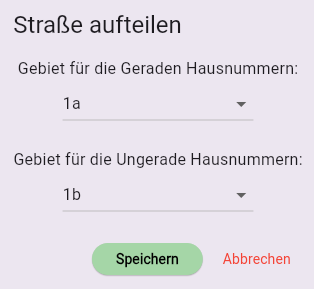
\includegraphics[width=\linewidth]{images/AdminPanel/splitStreetDialog.png}
        \caption{Dialog to split street}
    \end{minipage}
\end{figure}


The "Speichern" button triggers the \texttt{AdminAddressProvider} and shows a \texttt{Notification}(\ref{fig:Notification}) if the operation was successful or not. After that, the dialog is closed.

\lstset{style=mycsharp, caption=onPressed save button in splitStreetDialog}
\begin{lstlisting}
    int resultCode = await addressProvider.putAddressesOddEven(selectedAddresses.first.street.name, selectedAddresses.first.street.postalCode, selectedAreaEven, selectedAreaOdd);
    if (resultCode == 200) {
        showNotification("Adressen gespeichert", () => showAddressSavedNotification = true);
    } else {
        showNotification("Fehler beim Speichern", () => showAddAddressNotification = true);
    }
    if (!context.mounted) return;
    Navigator.of(context).pop();
\end{lstlisting}


\begin{figure}[H]
    \setstretch{1.5} % Erhöht den Zeilenabstand
    \centering
    \begin{minipage}{0.55\textwidth} % Linke Seite für den Text
        \subsubsection{Filter}
        With the Filter field, the administrator can filter the addresses displayed. It contains three dropdown menus to set the filter criteria, with one checkbox for each to toggle them. These filters can be combined as desired. 
    \end{minipage}
    \hfill 
    \begin{minipage}{0.4\textwidth} % Rechte Seite für das Bild
        \centering
        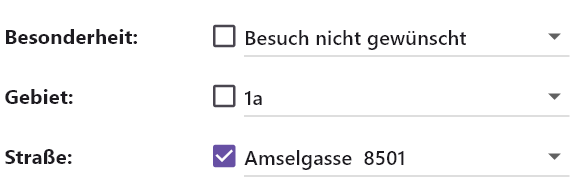
\includegraphics[width=\linewidth]{images/AdminPanel/FilterField.png}
        \caption{Filter field in AddressPage}
        \label{fig:adminpanel_filter}
    \end{minipage}
\end{figure}

The filter is passed and applied to the \texttt{MapComponent} and the \texttt{DatabaseViewComponent}. The criteria and their enabled/disabled state are managed by the following variables in the \texttt{AddressPage} class.
\lstset{style=mycsharp, caption=Filter variables in AddressPage}
\begin{lstlisting}
    bool specialFeatureFilter = false;
    bool areaFilter = false;
    bool streetFilter = false;
    
    String selectedStreetFilter = "";
    String selectedSpecialFeatureFilter = "";
    String selectedAreaFilter = "";
\end{lstlisting}

This is an example of how a \texttt{FilterRow} is defined in the \texttt{AddressPage} class (\ref{fig:FilterRow}):
\lstset{style=mycsharp, caption=FilterRow in AddressPage}
\begin{lstlisting}
    FilterRow(
        label: "Besonderheit:",
        tooltipMessage: "Besonderheitsfilter aktivieren/deaktivieren",
        filterValue: specialFeatureFilter,
        onFilterChanged: (bool? newValue) {
          setState(() => specialFeatureFilter = newValue ?? false);
        },
        selectedValue: selectedSpecialFeatureFilter,
        items: specialFeatureTextList,
        onDropdownChanged: (String? newValue) {
          setState(() => selectedSpecialFeatureFilter = newValue ?? "");
        },
      ),
\end{lstlisting}




 

\subsection{ListEditPage}
The \texttt{ListEditPage} is used to manage streets, special features and areas. 

\subsection{Components}


\subsubsection{MapComponent}


\paragraph{Edit multiple Addresses}

\label{fig:Select Street}
\paragraph{Select Street}

\paragraph{onClickNewAddress}

\paragraph{Select Coordinates on Map}


\subsubsection{DatabaseViewComponent}

\subsubsection{PDFSaver}

\subsubsection{AdminAddressProvider}

\subsubsection{CustomHttpClient}

\subsection{Models}

\subsubsection{AreaWithBorder}

\subsubsection{ScreenItem}

\subsection{Widgets}

\subsubsection{InputField}
\label{fig:InputField} 


\subsubsection{FilterRow}
\label{fig:FilterRow}